\documentclass{article}
% translate with >> pdflatex -shell-escape <file>

% This file is used as unit test for pgfplots, copyright by Christian Feuersaenger.
% 
% See
%   http://pgfplots.sourceforge.net/pgfplots.pdf
% for pgfplots.
%
% Any required input files (for <plot table> or <plot file> or the table package) can be downloaded
% at
% http://www.ctan.org/tex-archive/graphics/pgf/contrib/pgfplots/doc/latex/
% and
% http://www.ctan.org/tex-archive/graphics/pgf/contrib/pgfplots/doc/latex/plotdata/

\usepackage{pgfplots}
\pgfplotsset{compat=newest}

\pagestyle{empty}

\usepgfplotslibrary{ternary}

\begin{document}


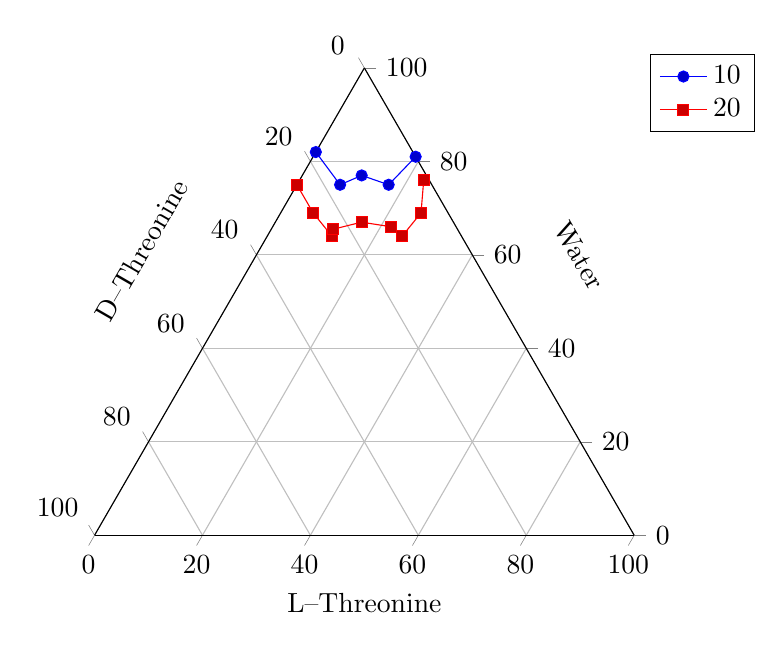
\begin{tikzpicture}
\begin{ternaryaxis}[
	xmax=100,ymax=100,zmax=100,
	ternary limits relative=false,
	%ternary start x=0.5,
	xlabel=Water,
	ylabel=D--Threonine,
	zlabel=L--Threonine,
	label style={sloped}
]
	\addplot3 coordinates {
		(82,	18,	0)
		(75,	17,	8)
		(77,	12,	11)
		(75,	8,	17)
		(81,	0,	19)
	};
	\addplot3 coordinates {
		(75,	25,	0)
		(69,	25,	6)
		(64,	24,	12)
		(65.5,	23,	11.5)
		(67,	17,	16)
		(66,	12,	22)
		(64,	11,	25)
		(69,	5,	26)
		(76,	1,	23)
	};
	\legend{$10$, $20$}
\end{ternaryaxis}
\end{tikzpicture}
\end{document}
